\documentclass{standalone}
\usepackage{pgfplots}
\pgfplotsset{compat=1.17}

\begin{document}

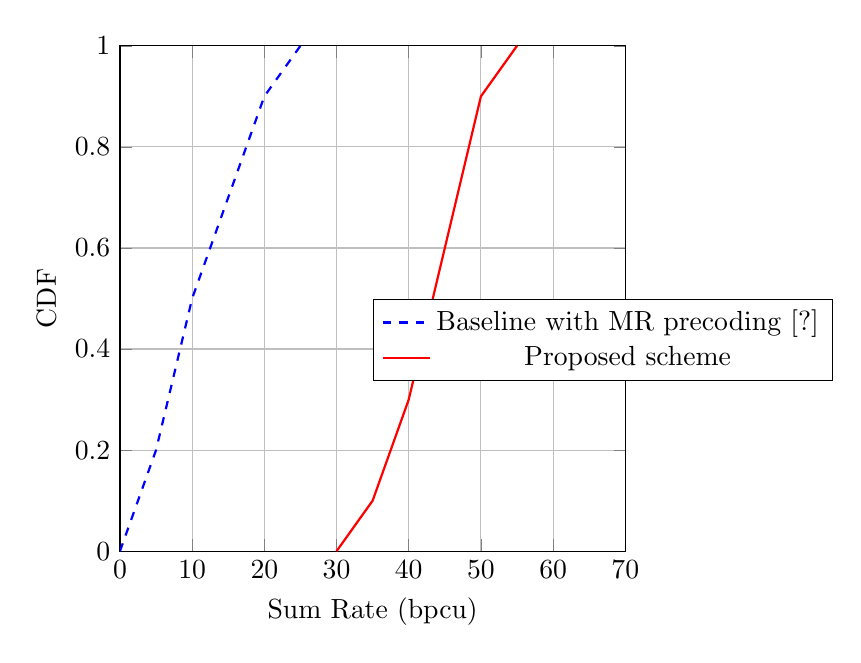
\begin{tikzpicture}
    \begin{axis}[
        width=8cm,
        height=8cm,
        xlabel={Sum Rate (bpcu)},
        ylabel={CDF},
        xmin=0, xmax=70,
        ymin=0, ymax=1,
        grid=both,
        legend style={at={(0.5,0.5)}, anchor=north west}
    ]
    
    % Baseline with MR precoding
    \addplot[blue, dashed, thick] coordinates {
        (0, 0) (5, 0.2) (10, 0.5) (15, 0.7) (20, 0.9) (25, 1)
    };
    \addlegendentry{Baseline with MR precoding [?]}
    
    % Proposed scheme
    \addplot[red, solid, thick] coordinates {
        (30, 0) (35, 0.1) (40, 0.3) (45, 0.6) (50, 0.9) (55, 1)
    };
    \addlegendentry{Proposed scheme}
    
    \end{axis}
\end{tikzpicture}

\end{document}